\documentclass[10pt,journal,onecolumn]{IEEEtran}
\usepackage{cite}
\usepackage{amsmath,amssymb,amsfonts,amsthm}
\usepackage{graphicx}
\usepackage{booktabs}
\usepackage{array}
\usepackage{xcolor}
\usepackage[hidelinks]{hyperref}
\newtheorem{proposition}{Proposition}
\newtheorem{remark}{Remark}
\renewcommand{\thesection}{S\arabic{section}}
\renewcommand{\thetable}{S\arabic{table}}
\renewcommand{\thefigure}{S\arabic{figure}}
\renewcommand{\theequation}{S\arabic{equation}}
\newcommand{\nSafeEpisodes}{1{,}800}
\newcommand{\safeMorePct}{0.0}


\begin{document}

\title{Supplementary Material for\\ ``IMBANG: Balancing DDoS Mitigation and Service Outages with Safety-Spanning Group-Relative Policy Optimisation''}

\author{Muntakimur~Rahaman, Azwan~Mahmud, and~Abdellah~Chehri}

\markboth{IEEE Networking Letters -- Supplementary Material}{IMBANG: Supplementary Material}

\maketitle

\section{Overview}
This document supports the letter with material that does not fit in four pages. It contains:
\begin{itemize}
\item the complete simulator, service model and symbolic shield that the letter adopts from Sentinel~\cite{alfatemi2026sentinel} (Sections~\ref{sec:s-sim} and~\ref{sec:s-shield});
\item full proofs of Propositions~1 and~2, and an empirical check of Proposition~2 over whole episodes (Section~\ref{sec:s-proofs});
\item every training and evaluation setting (Sections~\ref{sec:s-train} and~\ref{sec:s-eval});
\item extended results: all metrics with confidence intervals, all trained methods, paired tests, the red team, per-seed results and rule distillation (Sections~\ref{sec:s-results}--\ref{sec:s-interp});
\item the simulated operator study behind the ICMP limitation (Section~\ref{sec:s-human});
\item instructions for the accompanying code and data archive (Section~\ref{sec:s-repro}).
\end{itemize}
Tables, figures and equations here are numbered S1, S2, \dots; plain numbers such as ``Table~II'' refer to the letter. All results use seeds 42--51 and are paired with Sentinel's ten released checkpoints~\cite{sentinelcode}. Every number is generated from the per-seed files in the archive by \texttt{scripts/supp\_assets.py}.

The method's name, IMBANG, stands for \textbf{I}nterpretable, \textbf{M}onotone-safe, \textbf{B}udgeted, \textbf{A}dversary-free, \textbf{N}euro-symbolic \textbf{G}RPO. In the code and data files it is called \texttt{span}; Table~\ref{tab:s-names} lists all code names.

\begin{table}[!htbp]
\centering
\caption{Method Names in the Letter and in the Code}
\label{tab:s-names}
\small
\resizebox{\textwidth}{!}{%
\begin{tabular}{@{}lll@{}}
\toprule
Name in the letter & Code name & Description \\
\midrule
IMBANG & \texttt{span} & safe-side member + outage budget + MaxMC curriculum \\
C-GRPO & \texttt{span\_cgrpo} & outage budget with channel-wise cost normalisation~\cite{girgis2026cgrpo}, no safe-side member \\
IMBANG + C-GRPO norm. & \texttt{span\_cgrpo\_safe} & IMBANG with channel-wise cost normalisation \\
GRPO + budget & \texttt{span\_nosafe} & IMBANG without the safe-side member \\
\;\;+ entropy bonus $\times6$ & \texttt{span\_entropy} & GRPO + budget with six times the entropy weight \\
\;\;+ uncentred cost & \texttt{span\_abscost} & GRPO + budget with a cost advantage referenced to $\kappa$ instead of the group mean \\
MaxMC curriculum, no budget & \texttt{maxmc\_only} & curriculum only (extra baseline) \\
GRPO, no budget & \texttt{nscsd} & GRPO with archive curriculum, no budget \\
Plain GRPO & \texttt{grpo\_vanilla} & GRPO without archive, elites, anchor or shield tuning (Fig.~2 only) \\
PPO + shield & \texttt{ppo} & PPO with a critic, same shield and simulator budget \\
Sentinel & -- & released \texttt{best\_benchmark} checkpoints of~\cite{alfatemi2026sentinel} \\
\bottomrule
\end{tabular}}
\end{table}

% ===========================================================================
\section{Simulator and Service Model}
\label{sec:s-sim}
% ===========================================================================
The letter uses Sentinel's single-link simulator unchanged~\cite{alfatemi2026sentinel,sentinelcode}. We re-implemented it in batched form. Two tests in the archive (\texttt{tests/test\_env\_equivalence.py}) check that the port matches the reference code to within $10^{-5}$. Table~\ref{tab:s-repro} shows that Sentinel's released checkpoints reproduce its published results on our port. This section restates the model so that the proofs in Section~\ref{sec:s-proofs} can be checked line by line.

\textbf{Traffic.} The link capacity is $C=1000$ units per window. Benign traffic is $L_t\sim\mathrm{Poisson}(300)$; during a flash crowd it is multiplied by a factor drawn from $\mathcal{U}(2.5,4)$. The attack has a family $k_t\in\{\text{none},\text{SYN},\text{UDP},\text{HTTP},\text{ICMP},\text{mixed}\}$, an intensity $i_t\in[0,1]$ and a mutation level $m_t\in[0,1]$. Its volume is $A_t=1.5\,C\,i_t$, so a full-intensity flood alone exceeds the link by half.

\textbf{Action.} The defender chooses a load threshold $\tau_t\in(0,1)$, a filtering focus $f_t\in\{\text{SrcIP},\text{Proto},\text{Size}\}$ and a drop probability $d_t\in(0,1)$. Only the load above the threshold is filtered. The share of the offered load exposed to filtering is
\begin{equation}
\alpha_t(\tau)=\mathrm{clip}\!\left(\frac{L_t+A_t-C\tau}{L_t+A_t},\,0,\,1\right).
\end{equation}

\textbf{Effectiveness and collateral damage.} The match between focus and family is $\eta_t=\eta_{k_t f_t}\,(1-m_t/2)$, with the base values of Table~\ref{tab:s-match}. In an attacked window the shares of attack traffic dropped and of benign traffic lost are
\begin{align}
\mathrm{eff}_t &= \min\{1,\;\eta_t\,d_t\,\alpha_t(\tau_t)\},\\
\mathrm{CD}_t &= \min\Big\{1,\;0.4\,d_t\,(1-\eta_t)\,\alpha_t(\tau_t)+0.2\,\big[L_t-C\tau_t\big]^+/L_t\Big\}. \label{eq:s-cd}
\end{align}
Without an attack, the collateral damage is $\min\{1,\,0.05\,d_t\,\alpha_t(\tau_t)+0.1\,[L_t-C\tau_t]^+/L_t\}$. The leakage is $\mathrm{leak}_t=1-\mathrm{eff}_t$ in attacked windows.

\textbf{Service quality.} With the congestion factor $\rho_t=\min\{1,\,C/(L_t+A_t)\}$, computed on the offered (pre-filter) load,
\begin{equation}
\mathrm{SQ}_t=\rho_t\,(1-\mathrm{CD}_t). \label{eq:s-sq}
\end{equation}
A window is a \emph{severe outage} if $\mathrm{SQ}_t<0.5$ and \emph{degraded} if $\mathrm{SQ}_t<0.75$. Under a full-intensity flood, $\rho_t\approx1000/1800=0.556$, so even perfect filtering cannot lift service quality above 0.556, and a collateral damage of only about 0.10 already causes a severe outage.

\textbf{Score.} The operator's per-window composite score is Sentinel's benchmark,
\begin{equation}
b_t=\mathrm{SQ}_t-\mathrm{leak}_t-0.5\,\mathbf{1}[\mathrm{SQ}_t<0.5]-0.25\,\mathbf{1}[\mathrm{SQ}_t<0.75].
\end{equation}
All GRPO variants and the PPO baseline optimise $b_t$ directly. Sentinel's checkpoints were trained on its shaped reward and selected with $b_t$.

\textbf{Observation.} The defender observes twelve aggregate indicators of the served traffic in $[0,1]$: packet rate, byte rate, link utilisation, the TCP, UDP, ICMP and HTTP shares, the entropies of source address, destination port and packet size, a flow count and a queue (overload) signal. Small Gaussian noise is added to the protocol shares, the entropies and the packet rate. The protocol shares and entropies depend on the share of attack traffic that is served. The observation therefore depends on the previous action, which matters for the multi-step discussion in Section~\ref{sec:s-proofs}.

\begin{table}[!htbp]
\centering
\caption{Base Match Effectiveness $\eta_{kf}$ Between Attack Family and Filtering Focus~\cite{sentinelcode}}
\label{tab:s-match}
\small
\begin{tabular}{@{}lccc@{}}
\toprule
Family & SrcIP & Proto & Size \\
\midrule
SYN & 0.6 & 0.8 & 0.0 \\
UDP & 0.0 & 0.9 & 0.0 \\
HTTP & 0.7 & 0.0 & 0.5 \\
ICMP & 0.0 & 0.9 & 0.0 \\
Mixed & 0.4 & 0.4 & 0.4 \\
\bottomrule
\end{tabular}
\end{table}

\begin{table}[!htbp]
\centering
\caption{Sentinel's Released Checkpoints: Published Results and Our Port}
\label{tab:s-repro}
\small
\resizebox{\textwidth}{!}{%
\begin{tabular}{@{}lcccccc@{}}
\toprule
 & \multicolumn{2}{c}{Quality} & \multicolumn{2}{c}{Leakage} & \multicolumn{2}{c}{Severe / 500} \\
\cmidrule(lr){2-3}\cmidrule(lr){4-5}\cmidrule(l){6-7}
Scenario & Published & Port & Published & Port & Published & Port \\
\midrule
Benign & 1.000 & 1.000 & 0.000 & 0.000 & 0.0 & 0.0 \\
Chaos/flash crowd & 0.699 & 0.701 & 0.836 & 0.836 & 25.3 & 22.0 \\
Mild & 0.971 & 0.971 & 0.921 & 0.921 & 0.0 & 0.0 \\
Strong & 0.519 & 0.519 & 0.815 & 0.815 & 75.0 & 78.2 \\
Zero-shot ICMP & 0.529 & 0.529 & 0.747 & 0.747 & 0.0 & 0.0 \\
\bottomrule
\end{tabular}}
\vspace{2pt}
\parbox{\textwidth}{\footnotesize Published: Sentinel's evaluation tables. Port: our batched simulator with Sentinel's evaluation protocol and its released seed-42--51 checkpoints.}
\end{table}


% ===========================================================================
\section{Symbolic Shield}
\label{sec:s-shield}
% ===========================================================================
The shield $\mathcal{S}_\phi$ is Sentinel's rule set~\cite{alfatemi2026sentinel}, applied in the order of Table~\ref{tab:s-shield}. Each rule's trigger depends only on the observation $\mathbf{o}_t$ and on the proposed focus $f$. Each rule that changes $d$ or $\tau$ is a clamp of the form $\min\{\cdot,c\}$ or $\max\{\cdot,c\}$ with a constant $c$. IMBANG may tune the three PanicGuard constants $\phi=(g_u,g_d,g_\tau)$, defaults $(0.6,0.1,0.4)$, under the certificate described in Section~\ref{sec:s-train}. All other constants stay as in Sentinel.

\begin{table}[!htbp]
\centering
\caption{Shield Rules in Order of Application (util: link utilisation; src, size: entropies; udp, icmp, http: protocol shares)}
\label{tab:s-shield}
\small
\resizebox{\textwidth}{!}{%
\begin{tabular}{@{}clll@{}}
\toprule
\# & Rule & Trigger & Repair \\
\midrule
1 & PanicGuard (drop) & util $<g_u$ & $d\leftarrow\min\{d,\,g_d\}$ \\
2 & PanicGuard (threshold) & util $<g_u$ & $\tau\leftarrow\max\{\tau,\,g_\tau\}$ \\
3 & HTTP source-address exception & src $>0.85$, $f=$ SrcIP, util $>0.6$, http $>0.3$ & keep $f$ \\
4 & SpoofingGuard (protocol) & src $>0.85$, $f=$ SrcIP, util $>0.6$, rule 3 not met, a protocol share $>0.5$ & $f\leftarrow$ Proto \\
5 & SpoofingGuard (size) & as rule 4 but no protocol share $>0.5$ and size $<0.3$ & $f\leftarrow$ Size \\
6 & SpoofingGuard (fallback) & as rule 4 but no protocol share $>0.5$ and size $\ge0.3$ & $f\leftarrow$ Proto \\
7 & Protocol-anomaly guard & a protocol share $>0.8$, util $>0.6$, $f\ne$ Proto, not (http $>0.8$ and $f=$ SrcIP) & $f\leftarrow$ Proto \\
8 & ICMP focus override & icmp $>0.3$, util $>0.6$, $f\ne$ Proto & $f\leftarrow$ Proto \\
9 & ICMP drop override & icmp $>0.3$, util $>0.6$ & $d\leftarrow\max\{d,\,0.5\}$ \\
10 & ICMP threshold override & icmp $>0.3$, util $>0.6$ & $\tau\leftarrow\min\{\tau,\,0.5\}$ \\
11 & Extreme-drop cap & always & $d\leftarrow\min\{d,\,0.95\}$ \\
\bottomrule
\end{tabular}}
\end{table}

% ===========================================================================
\section{Proofs and an Empirical Check}
\label{sec:s-proofs}
% ===========================================================================
\textbf{Setting.} A GRPO group contains $G$ members that start from the same state and replay the same traffic, so they differ only in their actions. Member $g$ collects the objective $O_g=\sum_{h=1}^{H}b_h$ and the outage count $K_g=\sum_{h=1}^{H}\mathbf{1}[\mathrm{SQ}_h<0.5]$. With a multiplier $\lambda\ge0$, its return is $R_g=O_g-\lambda K_g$. The group-normalised advantage is
\begin{equation}
\hat A_g=\frac{R_g-\bar R}{s_R},\qquad \bar R=\frac1G\sum_{g'}R_{g'},\quad s_R=\Big(\frac1G\sum_{g'}(R_{g'}-\bar R)^2\Big)^{1/2},
\end{equation}
with $\hat A_g:=0$ when $s_R=0$.

\begin{proposition}[Constraint cancellation]
If $K_g\equiv K$ for every member of a group, then $\hat A_g$ does not depend on $\lambda$. The same holds for the channel-wise advantage $\hat A_g=\mathrm{z}(O)_g-\lambda\,\mathrm{z}(K)_g$ of Constrained GRPO~\cite{girgis2026cgrpo}, with the convention $\mathrm{z}(K)_g:=0$ when $s_K=0$.
\end{proposition}
\begin{proof}
If $K_g\equiv K$, then $\bar R=\bar O-\lambda K$, so $R_g-\bar R=O_g-\bar O$ for every $g$. The two sets of deviations coincide, so $s_R=s_O$ and $\hat A_g=(O_g-\bar O)/s_O$, which does not contain $\lambda$. For the channel-wise form, $K_g\equiv K$ gives $s_K=0$, hence $\mathrm{z}(K)\equiv0$ and $\hat A_g=\mathrm{z}(O)_g$.
\end{proof}

\begin{remark}
The argument uses only the fact that the advantage is invariant to adding the same constant to every return in a group. It therefore covers any group-centred advantage, with or without scaling. In such a group, the policy-gradient estimate is identical for every value of $\lambda$, so raising the multiplier cannot change the update. This is what Fig.~4 of the letter shows for ``budget only''. An \emph{uncentred} cost term, $\hat A_g-\lambda(K_g/H-\kappa)$, survives the centring but adds the same value to every member of such a group. In the clipped surrogate this shifts all sampled actions alike instead of pointing towards safer ones. This is consistent with the result in Table~\ref{tab:s-methods} that the uncentred cost does not restore feasibility.
\end{remark}

\begin{proposition}[Safe-side direction]
Let a policy member and the safe-side member observe the same $\mathbf{o}_t$ and face the same traffic in window $t$. The policy member proposes $(\tau,f,d)$, and the safe-side member executes $(\tilde\tau,\tilde f,\tilde d)=(\tau+(1-u)(1-\tau),\,f,\,u\,d)$ with $u\in[0.2,0.8]$. Then, after shielding, $\mathrm{CD}_t^{\mathrm{safe}}\le\mathrm{CD}_t^{\mathrm{policy}}$ and $\mathrm{SQ}_t^{\mathrm{safe}}\ge\mathrm{SQ}_t^{\mathrm{policy}}$. Consequently, the safe-side member is in a severe (or degraded) outage only if the policy member is.
\end{proposition}
\begin{proof}
\emph{(i) Before the shield.} Since $0\le u\le1$ and $\tau\le1$, we have $\tilde d=u\,d\le d$ and $\tilde\tau=\tau+(1-u)(1-\tau)\ge\tau$. Both stay in $[0,1]$.

\emph{(ii) Through the shield.} The rules that change the focus (3--8 in Table~\ref{tab:s-shield}) are triggered by $\mathbf{o}_t$ and the proposed focus only, and $\tilde f=f$. Both members therefore leave the shield with the same focus $f'$. Each rule acting on $d$ (1, 9, 11) has a trigger that depends on $\mathbf{o}_t$ only and applies $\min\{\cdot,c\}$ or $\max\{\cdot,c\}$. These maps are non-decreasing, and so is their composition. Hence $\tilde d\le d$ implies $\mathcal{S}(\tilde d)\le\mathcal{S}(d)$. The same argument applies to $\tau$ (rules 2 and 10) and gives $\mathcal{S}(\tilde\tau)\ge\mathcal{S}(\tau)$.

\emph{(iii) Through the service model.} With the same family, mutation and final focus $f'$, both members have the same $\eta_t$. In~\eqref{eq:s-cd}, $1-\eta_t\ge0$; $\alpha_t(\tau)$ and $[L_t-C\tau]^+$ are non-increasing in $\tau$; and the expression is non-decreasing in $d$. The no-attack expression has the same monotonicity, and $\min\{1,\cdot\}$ preserves it. Hence $\mathrm{CD}_t^{\mathrm{safe}}\le\mathrm{CD}_t^{\mathrm{policy}}$. Finally, $\rho_t$ in~\eqref{eq:s-sq} depends on the offered load only, not on the action, so $\mathrm{SQ}_t^{\mathrm{safe}}=\rho_t(1-\mathrm{CD}_t^{\mathrm{safe}})\ge\rho_t(1-\mathrm{CD}_t^{\mathrm{policy}})=\mathrm{SQ}_t^{\mathrm{policy}}$. Both outage indicators are monotone in $\mathrm{SQ}_t$.
\end{proof}

\textbf{Scope.} Proposition~2 is a statement about a single window, given the same observation. Two assumptions are structural. First, congestion is computed on the offered load. If filtering took place upstream of the bottleneck, a weaker filter could itself overload the link. Second, the shield acts through coordinate-wise clamps whose triggers do not depend on $d$ or $\tau$.

Over a rollout the two members' observations can diverge, because the protocol shares and entropies depend on how much attack traffic was served. A weaker filter serves more attack traffic, which can change later observations and hence later actions. The single-window guarantee therefore does not, by itself, imply an ordering of whole episodes.

We test the multi-step version empirically in Table~\ref{tab:s-safe}. Each trained IMBANG policy and its safe-shifted copy, with $u$ drawn once per episode, face identical traffic in all nine Protocol~B scenarios. In all \nSafeEpisodes\ episodes (ten seeds, nine scenarios, 20 episodes each), the safe copy had more severe windows than the policy in $\safeMorePct\%$ of episodes, that is, never. Under heavy floods it usually had fewer, and its episode-average collateral damage never exceeded the policy's. As the construction intends, it pays for this with higher leakage, which is why it serves as a training signal rather than as a deployed policy.

\begin{table}[!htbp]
\centering
\caption{Multi-Step Check of the Safe-Side Direction (IMBANG, Ten Seeds, 20 Episodes of 100 Windows)}
\label{tab:s-safe}
\small
\resizebox{\textwidth}{!}{%
\begin{tabular}{@{}lcccccccc@{}}
\toprule
 & \multicolumn{2}{c}{Severe / 500} & \multicolumn{2}{c}{Collateral damage} & \multicolumn{2}{c}{Leakage} & \multicolumn{2}{c}{Episodes (\%)} \\
\cmidrule(lr){2-3}\cmidrule(lr){4-5}\cmidrule(lr){6-7}\cmidrule(l){8-9}
Scenario & Policy & Safe & Policy & Safe & Policy & Safe & Safe fewer & Safe more \\
\midrule
Benign & 0.00 & 0.00 & 0.0000 & 0.0000 & 0.000 & 0.000 & 0.0 & 0.0 \\
Mild & 0.00 & 0.00 & 0.0187 & 0.0012 & 0.941 & 0.995 & 0.0 & 0.0 \\
Strong & 38.88 & 0.78 & 0.0633 & 0.0272 & 0.814 & 0.922 & 85.0 & 0.0 \\
Chaos/flash & 10.72 & 8.00 & 0.0386 & 0.0138 & 0.870 & 0.953 & 36.5 & 0.0 \\
ICMP (zero-shot) & 18.00 & 0.45 & 0.0541 & 0.0465 & 0.716 & 0.757 & 41.0 & 0.0 \\
Pulsing$^\ast$ & 16.05 & 0.40 & 0.0269 & 0.0123 & 0.847 & 0.933 & 73.5 & 0.0 \\
Polymorphic$^\ast$ & 14.23 & 0.38 & 0.0785 & 0.0308 & 0.890 & 0.957 & 93.0 & 0.0 \\
Boundary$^\ast$ & 0.00 & 0.00 & 0.0576 & 0.0142 & 0.835 & 0.959 & 0.0 & 0.0 \\
ICMP-chaos$^\ast$ & 20.88 & 17.48 & 0.0480 & 0.0283 & 0.800 & 0.873 & 34.5 & 0.0 \\
\bottomrule
\end{tabular}}
\vspace{2pt}
\parbox{\textwidth}{\footnotesize Each trained IMBANG policy and its safe-shifted copy ($\tilde d=u\,d$, $\tilde\tau=\tau+(1-u)(1-\tau)$, $u\sim\mathcal{U}(0.2,0.8)$ per episode) face identical traffic with the seeds of Protocol~B; the policy columns therefore equal Table~\ref{tab:s-b1}. Safe fewer / more: episodes in which the safe copy has strictly fewer / more severe windows.}
\end{table}


% ===========================================================================
\section{Training Details}
\label{sec:s-train}
% ===========================================================================
\textbf{Groups.} Each iteration samples $B=32$ training contexts, i.e.\ attack levels with their traffic. Each context is run for a random warm-up of 0--40 windows under the current policy and then forked into $G=8$ members that share all random numbers from the fork onwards~\cite{ng2000pegasus}. In IMBANG the members are:
\begin{itemize}
\item four ordinary policy samples;
\item one safe-side member: a policy sample transformed as in Proposition~2, with $u\sim\mathcal{U}(0.2,0.8)$ drawn once per rollout;
\item two shield probes: policy samples deployed under a perturbed PanicGuard;
\item one archive elite: the best stored solution for the level's niche, replaced by a policy sample when none exists.
\end{itemize}
Each member is rolled out for $H=8$ windows.

\textbf{Update.} The returns are $R_g=O_g-\lambda K_g$ and the advantages are group-normalised. Policy members and shield probes enter the clipped surrogate~\cite{schulman2017ppo}. The safe-side member and the elite enter only through the term
\begin{equation}
-c\,[\hat A_g]^+\log\pi_\theta(a_g\,|\,\mathbf{o}),\qquad c=0.5,
\end{equation}
so the policy moves towards them only when they outperformed their group. The loss also contains an entropy bonus and a KL penalty towards the best validated checkpoint (the anchor). It is minimised with Adam for four epochs per iteration. Table~\ref{tab:s-hyper} lists all values.

\textbf{Budget and selection.} Every 20 iterations the deterministic policy is evaluated on the validation battery (benign, mild, strong and chaos traffic; ten episodes of 100 windows each, with fixed random numbers). This gives the severe-outage rate $\hat\sigma$ and the validation score. The multiplier follows dual ascent, $\lambda\leftarrow[\lambda+\eta_\lambda(\hat\sigma-\kappa)]^+$, with $\eta_\lambda=4$ and $\kappa=0.05$. The deployed checkpoint is chosen lexicographically: any checkpoint that meets the budget beats every checkpoint that does not. Among feasible checkpoints the validation score decides; among infeasible ones, the lower outage rate does.

\textbf{Curriculum.} Training contexts come from 360 discrete levels: five family patterns (SYN, UDP, HTTP, mixed, switching), six intensity bands, three mutation bands, pulsing on or off, and flash crowds on or off. ICMP is excluded. At every validation round, each level is scored with the current policy (two episodes of 50 windows, fixed random numbers). Its MaxMC regret is the best score any earlier snapshot achieved on that level minus the current score~\cite{jiang2021robustplr}. With probability 0.5 a context is drawn from the prioritised-replay distribution of~\cite{jiang2021plr}: rank-based regret priority with temperature 0.3, mixed with a 0.3 share of staleness. Otherwise it is drawn uniformly over the levels.

\textbf{Certified shield tuning.} Every 20 iterations, eight PanicGuard candidates are proposed. Up to three lie along the direction accumulated from the shield probes' advantages; the rest are random perturbations. A candidate is adopted only if it meets three conditions:
\begin{itemize}
\item it improves the validation score by at least 0.002;
\item it keeps the validation outage rate within the budget;
\item it shows no safety regression against Sentinel's default shield on a certification battery of benign and flash-crowd traffic (ten episodes of 100 windows, fixed random numbers): service quality may not fall by more than 0.002 (benign) or 0.005 (flash crowd), and there may be no additional severe or degraded windows.
\end{itemize}
The certificate is empirical, not a formal guarantee.

\begin{table}[!htbp]
\centering
\caption{Hyperparameters (Fixed Before the Ten-Seed Runs)}
\label{tab:s-hyper}
\small
\resizebox{\textwidth}{!}{%
\begin{tabular}{@{}lll@{}}
\toprule
Setting & Value & Note \\
\midrule
\multicolumn{3}{@{}l}{\emph{GRPO learner (shared by all GRPO variants)}} \\
Iterations & 500 & validation every 20 iterations \\
Contexts per iteration $B$ / group size $G$ / horizon $H$ & 32 / 8 / 8 & warm-up 0--40 windows before the fork \\
Group composition (IMBANG) & 4 + 1 + 2 + 1 & policy samples, safe-side member, shield probes, archive elite \\
Optimiser & Adam, lr $0.0003$ & 4 epochs, minibatch 512, gradient-norm clip 0.5 \\
Clipping / entropy / KL-anchor weight & 0.2 / 0.005 / 0.02 & KL to the best validated checkpoint \\
Weight of the likelihood term $c$ & 0.5 & safe-side member and elite, $-c\,[\hat A]^+\log\pi_\theta$ \\
Objective & composite score $b_t$ & Sentinel's benchmark weights (severe 0.5, degraded 0.25) \\
\midrule
\multicolumn{3}{@{}l}{\emph{IMBANG-specific}} \\
Safe-side shift $u$ & $\mathcal{U}(0.2, 0.8)$ & drawn once per rollout \\
Outage budget $\kappa$ & 0.05 & severe-outage rate on the validation battery \\
Dual step $\eta_\lambda$ & 4.0 & per validation round, $\lambda_0=0$ \\
Champion selection & feasibility first & then composite validation score \\
Curriculum & MaxMC, 360 levels & 5 families $\times$ 6 intensity bands $\times$ 3 mutation bands $\times$ pulse $\times$ flash \\
Shield probes / perturbation & 2 / $\sigma=0.08$ & certified PanicGuard tuning \\
\midrule
\multicolumn{3}{@{}l}{\emph{Network and evaluation}} \\
Actor & 12--64--64 MLP & Beta heads for $\tau$ and $d$, categorical head for $f$ (Sentinel's architecture) \\
Seeds & 42--51 & paired with Sentinel's released checkpoints \\
Validation battery & benign, mild, strong, chaos & ICMP never seen before testing \\
Protocol B / A & 20 / 5 episodes & 100 windows each \\
Protocol C (red team) & CEM, 48 $\times$ 8 & 4 episodes of 60 windows per candidate; worst scenario re-scored on 20 fresh episodes of 100 \\
\bottomrule
\end{tabular}}
\end{table}


% ===========================================================================
\section{Evaluation Protocols and Statistics}
\label{sec:s-eval}
% ===========================================================================
\textbf{Protocol B (attacker-agnostic).} Nine open-loop scenarios (Table~\ref{tab:s-scen}), each with 20 episodes of 100 windows per seed. The first five mirror Sentinel's evaluation scenarios. The last four are held-out stress tests that were never used for training or model selection. ICMP traffic appears only at test time.

\textbf{Protocol A (Sentinel's own attackers).} For each seed, the attacker that Sentinel trained alongside its defender drives five scenarios with five episodes of 100 windows each, reproducing Sentinel's evaluation script. Averages in the letter and in Table~\ref{tab:s-a} are taken over the four attack scenarios and exclude benign traffic.

\textbf{Protocol C (red team).} A cross-entropy search explores the full 14-dimensional scenario space, ICMP included:
\begin{itemize}
\item eight iterations of 48 candidates;
\item each candidate scored on four episodes of 60 windows;
\item the elite is the best 20\%.
\end{itemize}
The worst scenario found is then re-scored on 20 fresh episodes of 100 windows.

\textbf{Common random numbers and statistics.} For a given seed and scenario, all defenders face identical traffic, so comparisons are paired by seed. We report means with 95\% $t$-intervals over the ten seeds. The tests are paired $t$-tests with Holm correction across the eight attack scenarios for each metric, and two-sided Wilcoxon signed-rank tests. With ten pairs, the smallest attainable Wilcoxon $p$-value is 0.002.

\begin{table}[!htbp]
\centering
\caption{Protocol~B Evaluation Scenarios}
\label{tab:s-scen}
\small
\resizebox{\textwidth}{!}{%
\begin{tabular}{@{}lp{4.2cm}cccccl@{}}
\toprule
Scenario & Attack families (weights) & Persistence & Intensity & Mutation & Pulse period / duty & Flash prob. & Role \\
\midrule
Benign & none & 0.95 & [0.0, 0.0] & [0.0, 1.0] & -- & 0.00 & Sentinel scenario \\
Mild & SYN, UDP, HTTP, mixed & 0.95 & [0.0, 0.3] & [0.0, 1.0] & -- & 0.00 & Sentinel scenario \\
Strong & SYN, UDP, HTTP, mixed & 0.95 & [1.0, 1.0] & [0.0, 1.0] & -- & 0.00 & Sentinel scenario \\
Chaos/flash & none, SYN, UDP, HTTP, mixed & 0.95 & [0.0, 1.0] & [0.0, 1.0] & -- & 0.05 & Sentinel scenario \\
ICMP (zero-shot) & ICMP & 0.95 & [1.0, 1.0] & [0.0, 1.0] & -- & 0.00 & Sentinel scenario (unseen family) \\
Pulsing$^\ast$ & SYN, UDP, HTTP, mixed & 0.95 & [1.0, 1.0] & [0.0, 1.0] & 10 / 0.5 & 0.00 & held-out stress test \\
Polymorphic$^\ast$ & SYN, UDP, HTTP, mixed & 0.50 & [0.5, 1.0] & [0.7, 1.0] & -- & 0.00 & held-out stress test \\
Boundary$^\ast$ & SYN, UDP, HTTP, mixed & 0.95 & [0.3, 0.6] & [0.0, 1.0] & -- & 0.00 & held-out stress test \\
ICMP-chaos$^\ast$ & none (0.12), SYN (0.12), UDP (0.12), HTTP (0.12), ICMP (0.38), mixed (0.12) & 0.95 & [0.5, 1.0] & [0.0, 1.0] & -- & 0.05 & held-out stress test \\
\bottomrule
\end{tabular}}
\vspace{2pt}
\parbox{\textwidth}{\footnotesize Families switch with probability $1-$persistence per window; intensity and mutation are redrawn uniformly from their ranges on each switch. $^\ast$Never used for training or model selection.}
\end{table}


% ===========================================================================
\section{Extended Results}
\label{sec:s-results}
% ===========================================================================
Tables~\ref{tab:s-b1} and~\ref{tab:s-b2} extend Table~II of the letter with confidence intervals, service quality, leakage and the PPO baseline. Table~\ref{tab:s-tests} gives the paired tests behind the significance marks. Table~\ref{tab:s-a} reports Protocol~A by scenario, and Table~\ref{tab:s-methods} compares all trained methods across the three protocols. Fig.~\ref{fig:s-seeds} shows the seed-level pairs: IMBANG scores higher than Sentinel on every seed and has a far narrower spread of outages. Fig.~\ref{fig:s-scen} breaks the severe outages down by scenario.

Table~\ref{tab:s-methods} also lists the four reference heuristics shipped with Sentinel's code. They show why the outage count alone is not a sufficient measure. Sentinel's adaptive heuristic matches IMBANG's outage count (14.5 against 14.8 per 500 windows), but only because it filters very little: it lets 96.9\% of the attack traffic through, against 83.9\% for IMBANG. Its composite score is lower than that of every learned defender.

\begin{table}[!htbp]
\centering
\caption{Protocol~B: Composite Score and Severe Outages per 500 Windows (Mean $\pm$ 95\% CI over Ten Seeds)}
\label{tab:s-b1}
\small
\resizebox{\textwidth}{!}{%
\begin{tabular}{@{}lcccccccc@{}}
\toprule
 & \multicolumn{4}{c}{Composite score $\uparrow$} & \multicolumn{4}{c}{Severe outages $\downarrow$} \\
\cmidrule(lr){2-5}\cmidrule(l){6-9}
Scenario & Sentinel & PPO & C-GRPO & IMBANG & Sentinel & PPO & C-GRPO & IMBANG \\
\midrule
Benign & $1.000\pm0.000$ & $1.000\pm0.000$ & $1.000\pm0.000$ & $1.000\pm0.000$ & $0.0\pm0.0$ & $0.0\pm0.0$ & $0.0\pm0.0$ & $0.0\pm0.0$ \\
Mild & $0.009\pm0.003$ & $0.008\pm0.003$ & $0.053\pm0.014$ & $0.040\pm0.006$ & $0.0\pm0.0$ & $0.0\pm0.0$ & $0.0\pm0.0$ & $0.0\pm0.0$ \\
Strong & $-0.746\pm0.066$ & $-0.647\pm0.038$ & $-0.612\pm0.048$ & $-0.583\pm0.018$ & $155.2\pm49.9$ & $83.4\pm37.8$ & $85.9\pm59.9$ & $38.9\pm14.6$ \\
Chaos/flash & $-0.169\pm0.019$ & $-0.150\pm0.021$ & $-0.114\pm0.018$ & $-0.123\pm0.020$ & $14.1\pm2.3$ & $10.6\pm1.4$ & $16.8\pm9.9$ & $10.7\pm1.2$ \\
ICMP (zero-shot) & $-0.474\pm0.010$ & $-0.467\pm0.012$ & $-0.474\pm0.008$ & $-0.458\pm0.020$ & $4.6\pm9.3$ & $3.7\pm4.1$ & $23.3\pm35.5$ & $18.0\pm17.3$ \\
Pulsing$^\ast$ & $-0.303\pm0.026$ & $-0.250\pm0.008$ & $-0.228\pm0.017$ & $-0.225\pm0.009$ & $60.5\pm20.1$ & $27.9\pm10.0$ & $37.7\pm27.2$ & $16.1\pm5.8$ \\
Polymorphic$^\ast$ & $-0.454\pm0.008$ & $-0.442\pm0.009$ & $-0.442\pm0.014$ & $-0.430\pm0.008$ & $14.9\pm6.1$ & $10.5\pm3.6$ & $24.0\pm12.9$ & $14.2\pm3.4$ \\
Boundary$^\ast$ & $0.003\pm0.012$ & $0.017\pm0.005$ & $0.084\pm0.018$ & $0.071\pm0.018$ & $0.0\pm0.0$ & $0.0\pm0.0$ & $0.0\pm0.0$ & $0.0\pm0.0$ \\
ICMP-chaos$^\ast$ & $-0.299\pm0.024$ & $-0.276\pm0.022$ & $-0.255\pm0.030$ & $-0.257\pm0.022$ & $25.4\pm4.1$ & $21.1\pm2.4$ & $25.2\pm5.2$ & $20.9\pm1.8$ \\
\midrule
Average (attacks) & $-0.304\pm0.014$ & $-0.276\pm0.006$ & $-0.248\pm0.009$ & $-0.246\pm0.009$ & $34.4\pm9.5$ & $19.6\pm6.8$ & $26.6\pm17.8$ & $14.8\pm3.3$ \\
\bottomrule
\end{tabular}}
\vspace{2pt}
\parbox{\textwidth}{\footnotesize $^\ast$Held-out stress test. Severe outages are windows with service quality below 0.5. PPO: PPO + shield trained with the same budget of simulator windows.}
\end{table}

\begin{table}[!htbp]
\centering
\caption{Protocol~B: Service Quality and Attack Leakage (Mean $\pm$ 95\% CI over Ten Seeds)}
\label{tab:s-b2}
\small
\resizebox{\textwidth}{!}{%
\begin{tabular}{@{}lcccccccc@{}}
\toprule
 & \multicolumn{4}{c}{Service quality $\uparrow$} & \multicolumn{4}{c}{Attack leakage $\downarrow$} \\
\cmidrule(lr){2-5}\cmidrule(l){6-9}
Scenario & Sentinel & PPO & C-GRPO & IMBANG & Sentinel & PPO & C-GRPO & IMBANG \\
\midrule
Benign & $1.000\pm0.000$ & $1.000\pm0.000$ & $1.000\pm0.000$ & $1.000\pm0.000$ & $0.000\pm0.000$ & $0.000\pm0.000$ & $0.000\pm0.000$ & $0.000\pm0.000$ \\
Mild & $0.991\pm0.002$ & $0.994\pm0.002$ & $0.970\pm0.004$ & $0.981\pm0.004$ & $0.983\pm0.004$ & $0.986\pm0.004$ & $0.917\pm0.017$ & $0.941\pm0.009$ \\
Strong & $0.511\pm0.005$ & $0.516\pm0.003$ & $0.513\pm0.006$ & $0.520\pm0.002$ & $0.852\pm0.025$ & $0.829\pm0.011$ & $0.789\pm0.027$ & $0.814\pm0.018$ \\
Chaos/flash & $0.837\pm0.011$ & $0.842\pm0.011$ & $0.829\pm0.012$ & $0.838\pm0.012$ & $0.908\pm0.017$ & $0.899\pm0.016$ & $0.843\pm0.014$ & $0.870\pm0.018$ \\
ICMP (zero-shot) & $0.529\pm0.002$ & $0.528\pm0.002$ & $0.526\pm0.004$ & $0.526\pm0.003$ & $0.748\pm0.019$ & $0.742\pm0.015$ & $0.727\pm0.035$ & $0.716\pm0.029$ \\
Pulsing$^\ast$ & $0.759\pm0.002$ & $0.761\pm0.001$ & $0.760\pm0.003$ & $0.763\pm0.001$ & $0.877\pm0.016$ & $0.858\pm0.010$ & $0.825\pm0.018$ & $0.847\pm0.009$ \\
Polymorphic$^\ast$ & $0.657\pm0.006$ & $0.660\pm0.006$ & $0.647\pm0.010$ & $0.662\pm0.004$ & $0.905\pm0.010$ & $0.902\pm0.007$ & $0.868\pm0.016$ & $0.890\pm0.008$ \\
Boundary$^\ast$ & $0.914\pm0.007$ & $0.922\pm0.006$ & $0.893\pm0.008$ & $0.907\pm0.007$ & $0.908\pm0.011$ & $0.905\pm0.006$ & $0.807\pm0.019$ & $0.835\pm0.021$ \\
ICMP-chaos$^\ast$ & $0.710\pm0.010$ & $0.714\pm0.010$ & $0.710\pm0.009$ & $0.715\pm0.009$ & $0.829\pm0.018$ & $0.816\pm0.014$ & $0.783\pm0.030$ & $0.800\pm0.018$ \\
\midrule
Average (attacks) & $0.738\pm0.003$ & $0.742\pm0.002$ & $0.731\pm0.005$ & $0.739\pm0.003$ & $0.876\pm0.013$ & $0.867\pm0.008$ & $0.820\pm0.016$ & $0.839\pm0.013$ \\
\bottomrule
\end{tabular}}
\vspace{2pt}
\parbox{\textwidth}{\footnotesize $^\ast$Held-out stress test. Severe outages are windows with service quality below 0.5. PPO: PPO + shield trained with the same budget of simulator windows.}
\end{table}

\begin{table}[!htbp]
\centering
\caption{Paired Tests over Ten Seeds (Protocol~B)}
\label{tab:s-tests}
\small
\resizebox{\textwidth}{!}{%
\begin{tabular}{@{}lcccccccc@{}}
\toprule
 & \multicolumn{4}{c}{Composite score} & \multicolumn{4}{c}{Severe outages / 500} \\
\cmidrule(lr){2-5}\cmidrule(l){6-9}
Scenario & $\Delta$ & Holm $p$ & Wilcoxon $p$ & $d_z$ & $\Delta$ & Holm $p$ & Wilcoxon $p$ & $d_z$ \\
\midrule
\multicolumn{9}{@{}l}{\emph{IMBANG vs Sentinel}} \\
Mild & +0.031 & $1.1\times10^{-6}$ & $2.0\times10^{-3}$ & +4.65 & +0.0 & 1.00 & 1.00 & +0.00 \\
Strong & +0.164 & $2.7\times10^{-4}$ & $2.0\times10^{-3}$ & +2.20 & -116.3 & $3.5\times10^{-3}$ & $3.9\times10^{-3}$ & -1.71 \\
Chaos/flash & +0.046 & $1.3\times10^{-4}$ & $2.0\times10^{-3}$ & +2.55 & -3.4 & 0.09 & 0.04 & -0.94 \\
ICMP (zero-shot) & +0.016 & 0.04 & 0.04 & +0.78 & +13.4 & 0.57 & 0.08 & +0.51 \\
Pulsing$^\ast$ & +0.078 & $5.2\times10^{-4}$ & $2.0\times10^{-3}$ & +1.94 & -44.5 & $5.9\times10^{-3}$ & $3.9\times10^{-3}$ & -1.55 \\
Polymorphic$^\ast$ & +0.024 & $2.1\times10^{-4}$ & $2.0\times10^{-3}$ & +2.33 & -0.6 & 1.00 & 0.98 & -0.06 \\
Boundary$^\ast$ & +0.068 & $6.1\times10^{-5}$ & $2.0\times10^{-3}$ & +2.84 & +0.0 & 1.00 & 1.00 & +0.00 \\
ICMP-chaos$^\ast$ & +0.042 & $5.9\times10^{-3}$ & $5.9\times10^{-3}$ & +1.27 & -4.6 & 0.12 & 0.02 & -0.86 \\
\midrule
\multicolumn{9}{@{}l}{\emph{IMBANG vs C-GRPO}} \\
Mild & -0.013 & 0.28 & 0.05 & -0.78 & +0.0 & 1.00 & 1.00 & +0.00 \\
Strong & +0.029 & 0.37 & 0.02 & +0.62 & -47.0 & 0.66 & 0.04 & -0.62 \\
Chaos/flash & -0.009 & 0.37 & 0.05 & -0.64 & -6.0 & 0.81 & $9.8\times10^{-3}$ & -0.43 \\
ICMP (zero-shot) & +0.016 & 0.35 & 0.11 & +0.69 & -5.3 & 1.00 & 0.65 & -0.10 \\
Pulsing$^\ast$ & +0.003 & 1.00 & 0.70 & +0.13 & -21.6 & 0.70 & $5.9\times10^{-3}$ & -0.58 \\
Polymorphic$^\ast$ & +0.012 & 0.32 & $3.9\times10^{-3}$ & +0.73 & -9.8 & 0.80 & 0.05 & -0.48 \\
Boundary$^\ast$ & -0.013 & 0.37 & 0.11 & -0.63 & +0.0 & 1.00 & 1.00 & +0.00 \\
ICMP-chaos$^\ast$ & -0.002 & 1.00 & 1.00 & -0.06 & -4.3 & 0.70 & $3.9\times10^{-3}$ & -0.57 \\
\bottomrule
\end{tabular}}
\vspace{2pt}
\parbox{\textwidth}{\footnotesize $\Delta$: IMBANG minus comparator, averaged over seeds. Holm: paired $t$-test, Holm-corrected across the eight scenarios per metric. Wilcoxon: signed-rank test (two-sided, uncorrected; its smallest attainable value with ten pairs is 0.002). $d_z$: standardised paired effect size.}
\end{table}

\begin{table}[!htbp]
\centering
\caption{Protocol~A: Sentinel's Own Trained Attackers (Ten Seeds, Five Episodes Each)}
\label{tab:s-a}
\small
\resizebox{\textwidth}{!}{%
\begin{tabular}{@{}lcccccccc@{}}
\toprule
 & \multicolumn{2}{c}{Composite $\uparrow$} & \multicolumn{2}{c}{Severe / 500 $\downarrow$} & \multicolumn{2}{c}{Leakage $\downarrow$} & \multicolumn{2}{c}{Quality $\uparrow$} \\
\cmidrule(lr){2-3}\cmidrule(lr){4-5}\cmidrule(lr){6-7}\cmidrule(l){8-9}
Scenario & Sentinel & IMBANG & Sentinel & IMBANG & Sentinel & IMBANG & Sentinel & IMBANG \\
\midrule
Benign & $1.000\pm0.000$ & $1.000\pm0.000$ & $0.0\pm0.0$ & $0.0\pm0.0$ & 0.000 & 0.000 & 1.000 & 1.000 \\
Mild & $0.051\pm0.035$ & $0.141\pm0.062$ & $0.0\pm0.0$ & $0.0\pm0.0$ & 0.921 & 0.808 & 0.971 & 0.950 \\
Strong & $-0.625\pm0.193$ & $-0.509\pm0.069$ & $78.2\pm123.0$ & $5.5\pm8.3$ & 0.815 & 0.778 & 0.519 & 0.524 \\
Chaos/flash crowd & $-0.288\pm0.150$ & $-0.251\pm0.144$ & $22.0\pm4.3$ & $19.8\pm5.8$ & 0.836 & 0.811 & 0.701 & 0.711 \\
Zero-shot ICMP & $-0.468\pm0.029$ & $-0.439\pm0.033$ & $0.0\pm0.0$ & $0.0\pm0.0$ & 0.747 & 0.715 & 0.529 & 0.526 \\
\midrule
Average (attacks) & $-0.332\pm0.062$ & $-0.265\pm0.039$ & $25.1\pm30.5$ & $6.3\pm3.1$ & 0.830 & 0.778 & 0.680 & 0.678 \\
\bottomrule
\end{tabular}}
\vspace{2pt}
\parbox{\textwidth}{\footnotesize For each seed, the attacker that Sentinel co-trained with its defender drives the traffic, as in Sentinel's own evaluation script; for IMBANG this is a transfer test. Leakage is averaged over all windows. Paired $t$-tests on the attack average: composite $p=0.019$, severe $p=0.22$, leakage $p=0.018$, quality $p=0.65$.}
\end{table}

\begin{table}[!htbp]
\centering
\caption{All Trained Methods (Ten Seeds; Protocol~B Averaged over the Eight Attack Scenarios)}
\label{tab:s-methods}
\small
\resizebox{\textwidth}{!}{%
\begin{tabular}{@{}lccccccccc@{}}
\toprule
Method & Composite (B) & Severe (B) & Leakage (B) & Quality (B) & Composite (A) & Worst (C) & Budget met & Final $\lambda$ & Span rate \\
\midrule
Sentinel & $-0.304\pm0.014$ & $34.4\pm9.5$ & 0.876 & 0.738 & -0.332 & $-1.07\pm0.17$ & -- & -- & -- \\
PPO + shield & $-0.276\pm0.006$ & $19.6\pm6.8$ & 0.867 & 0.742 & -0.315 & $-0.79\pm0.09$ & -- & -- & -- \\
GRPO, no budget & $-0.250\pm0.009$ & $91.5\pm24.2$ & 0.729 & 0.710 & -0.276 & $-1.07\pm0.08$ & -- & -- & -- \\
MaxMC curriculum, no budget & $-0.244\pm0.010$ & $52.4\pm25.9$ & 0.777 & 0.721 & -0.246 & $-0.88\pm0.12$ & 0/10 & 0.00 & 0.42 \\
GRPO + budget & $-0.253\pm0.011$ & $36.5\pm19.9$ & 0.812 & 0.729 & -0.248 & $-0.87\pm0.15$ & 1/10 & 7.69 & 0.43 \\
\;\;+ entropy bonus $\times6$ & $-0.249\pm0.010$ & $33.8\pm19.4$ & 0.810 & 0.729 & -0.244 & $-0.85\pm0.16$ & 0/10 & 7.54 & 0.43 \\
\;\;+ uncentred cost & $-0.251\pm0.010$ & $34.7\pm19.3$ & 0.812 & 0.730 & -0.242 & $-0.87\pm0.13$ & 1/10 & 7.38 & 0.44 \\
C-GRPO & $-0.248\pm0.009$ & $26.6\pm17.8$ & 0.820 & 0.731 & -0.262 & $-0.80\pm0.13$ & 3/10 & 4.67 & 0.36 \\
\textbf{IMBANG} & $-0.246\pm0.009$ & $14.8\pm3.3$ & 0.839 & 0.739 & -0.265 & $-0.72\pm0.03$ & 9/10 & 0.43 & 0.42 \\
IMBANG + C-GRPO norm. & $-0.247\pm0.007$ & $12.1\pm2.5$ & 0.843 & 0.739 & -0.266 & $-0.71\pm0.02$ & 7/10 & 0.41 & 0.42 \\
\midrule
\multicolumn{10}{@{}l}{\emph{Reference heuristics from Sentinel's code (no learning)}} \\
Adaptive heuristic & $-0.342\pm0.004$ & $14.5\pm0.9$ & 0.969 & 0.766 & -0.431 & $-0.71\pm0.01$ & -- & -- & -- \\
Static rule & $-0.319\pm0.005$ & $24.8\pm2.5$ & 0.916 & 0.751 & -0.385 & $-0.88\pm0.09$ & -- & -- & -- \\
Random actions + shield & $-0.388\pm0.004$ & $86.1\pm1.4$ & 0.875 & 0.714 & -0.471 & $-0.93\pm0.02$ & -- & -- & -- \\
Random actions & $-0.476\pm0.004$ & $109.8\pm1.3$ & 0.920 & 0.698 & -0.610 & $-0.97\pm0.03$ & -- & -- & -- \\
\bottomrule
\end{tabular}}
\vspace{2pt}
\parbox{\textwidth}{\footnotesize Worst (C): composite score of the worst scenario found by the red team. Budget met: seeds whose final validation outage rate is at most $\kappa=0.05$. Span rate: share of training groups whose members differ in outage count, averaged over the last 100 iterations. --: not applicable or not logged. Adaptive: Sentinel's traffic-responsive heuristic; Static: fixed protocol filtering (threshold 0.8, drop 0.5).}
\end{table}


\begin{figure}[!htbp]
\centering
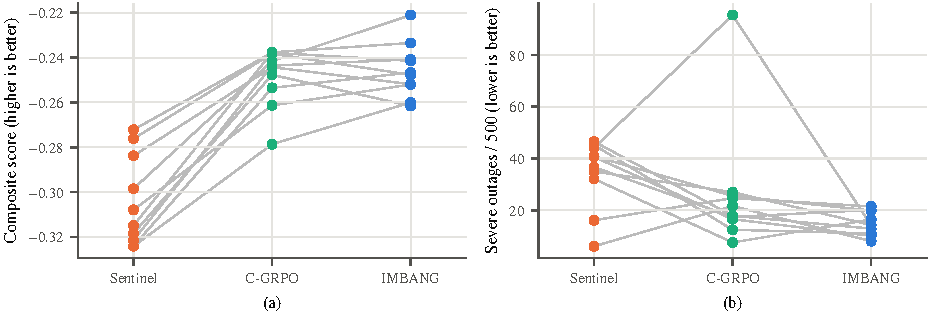
\includegraphics[width=0.85\textwidth]{figures/seeds.pdf}
\caption{Seed-level comparison under Protocol~B (scenario average over the eight attack scenarios). Grey lines connect the same seed. (a) Composite score. (b) Severe outages per 500 windows.}
\label{fig:s-seeds}
\end{figure}

\begin{figure}[!htbp]
\centering
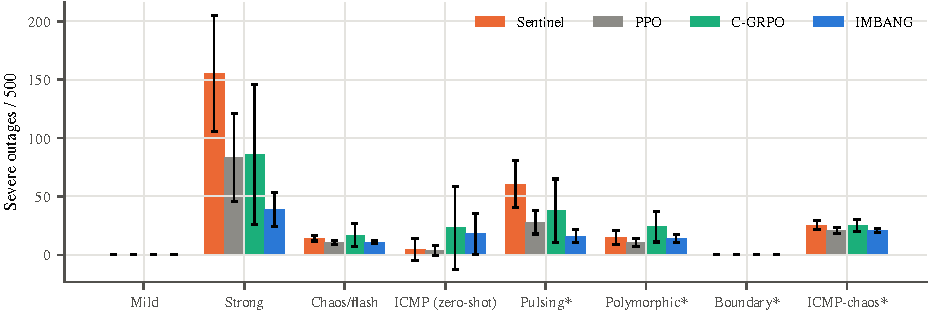
\includegraphics[width=0.85\textwidth]{figures/scenarios.pdf}
\caption{Severe outages per 500 windows by Protocol~B scenario (mean and 95\% confidence interval over ten seeds; $\ast$ marks held-out stress tests).}
\label{fig:s-scen}
\end{figure}

\textbf{Red team.} Table~\ref{tab:s-redteam} details the worst cases. For Sentinel the search most often settles on HTTP floods; for the PPO and GRPO-trained defenders it mostly settles on mixed floods. Among learned defenders, IMBANG and its variant with C-GRPO normalisation have the best worst cases ($-0.72$ and $-0.71$) and the smallest spread across seeds. Sentinel's adaptive heuristic reaches a similar worst case ($-0.71$), but its average leakage is far higher (Table~\ref{tab:s-methods}).

\begin{table}[!htbp]
\centering
\caption{Protocol~C: Worst Case Found by the Cross-Entropy Red Team (Ten Seeds)}
\label{tab:s-redteam}
\small
\resizebox{\textwidth}{!}{%
\begin{tabular}{@{}lcccccl@{}}
\toprule
Method & Worst composite & Severe / 500 & Quality & Leakage & Intensity & Worst family (seeds) \\
\midrule
Sentinel & $-1.07\pm0.17$ & $359.6\pm127.3$ & 0.494 & 0.960 & 0.98 & http 7, mixed 3 \\
PPO + shield & $-0.79\pm0.09$ & $141.4\pm84.4$ & 0.505 & 0.909 & 0.97 & mixed 9, syn 1 \\
GRPO, no budget & $-1.07\pm0.08$ & $466.6\pm37.7$ & 0.462 & 0.821 & 0.97 & mixed 7, http 2, syn 1 \\
MaxMC curriculum, no budget & $-0.88\pm0.12$ & $254.3\pm127.1$ & 0.487 & 0.868 & 0.97 & mixed 7, http 2, syn 1 \\
GRPO + budget & $-0.87\pm0.15$ & $213.0\pm151.4$ & 0.500 & 0.908 & 0.97 & mixed 9, udp 1 \\
\;\;+ entropy bonus $\times6$ & $-0.85\pm0.16$ & $208.7\pm161.1$ & 0.501 & 0.893 & 0.97 & mixed 9, syn 1 \\
\;\;+ uncentred cost & $-0.87\pm0.13$ & $214.3\pm132.5$ & 0.502 & 0.907 & 0.97 & mixed 10 \\
C-GRPO & $-0.80\pm0.13$ & $155.5\pm121.3$ & 0.505 & 0.905 & 0.97 & mixed 9, http 1 \\
\textbf{IMBANG} & $-0.72\pm0.03$ & $67.8\pm46.3$ & 0.521 & 0.921 & 0.96 & mixed 8, http 1, udp 1 \\
IMBANG + C-GRPO norm. & $-0.71\pm0.02$ & $46.4\pm24.3$ & 0.523 & 0.935 & 0.97 & mixed 8, http 2 \\
\midrule
Adaptive heuristic & $-0.71\pm0.01$ & $29.4\pm2.0$ & 0.558 & 0.995 & 0.96 & http 8, mixed 2 \\
Static rule & $-0.88\pm0.09$ & $150.1\pm80.7$ & 0.509 & 0.988 & 0.97 & http 10 \\
Random actions + shield & $-0.93\pm0.02$ & $253.7\pm15.0$ & 0.486 & 0.919 & 0.97 & http 6, mixed 4 \\
Random actions & $-0.97\pm0.03$ & $263.7\pm16.6$ & 0.479 & 0.935 & 0.97 & udp 6, icmp 3, http 1 \\
\bottomrule
\end{tabular}}
\vspace{2pt}
\parbox{\textwidth}{\footnotesize The red team searches the full 14-dimensional scenario space, ICMP included, for the scenario that minimises each defender's composite score.}
\end{table}


\textbf{Operating curve.} Table~\ref{tab:s-int} lists the data of Fig.~3 of the letter.

\begin{table}[!htbp]
\centering
\caption{Operating Curve over Attack Intensity (Data of Fig.~3 of the Letter)}
\label{tab:s-int}
\small
\resizebox{\textwidth}{!}{%
\begin{tabular}{@{}cccccccccc@{}}
\toprule
 & \multicolumn{3}{c}{Severe / 500 $\downarrow$} & \multicolumn{3}{c}{Leakage $\downarrow$} & \multicolumn{3}{c}{Quality $\uparrow$} \\
\cmidrule(lr){2-4}\cmidrule(lr){5-7}\cmidrule(l){8-10}
Intensity & Sentinel & C-GRPO & IMBANG & Sentinel & C-GRPO & IMBANG & Sentinel & C-GRPO & IMBANG \\
\midrule
0.10 & 0.0 & 0.0 & 0.0 & 1.000 & 0.980 & 0.998 & 1.000 & 0.993 & 1.000 \\
0.20 & 0.0 & 0.0 & 0.0 & 0.984 & 0.882 & 0.917 & 0.991 & 0.953 & 0.971 \\
0.30 & 0.0 & 0.0 & 0.0 & 0.938 & 0.814 & 0.842 & 0.965 & 0.929 & 0.944 \\
0.40 & 0.0 & 0.0 & 0.0 & 0.915 & 0.776 & 0.794 & 0.951 & 0.916 & 0.926 \\
0.50 & 0.0 & 0.0 & 0.0 & 0.895 & 0.830 & 0.878 & 0.898 & 0.896 & 0.915 \\
0.60 & 0.0 & 0.0 & 0.0 & 0.879 & 0.818 & 0.861 & 0.781 & 0.780 & 0.796 \\
0.70 & 0.0 & 0.0 & 0.0 & 0.869 & 0.808 & 0.845 & 0.690 & 0.691 & 0.703 \\
0.80 & 0.0 & 0.1 & 0.1 & 0.860 & 0.795 & 0.827 & 0.618 & 0.620 & 0.629 \\
0.86 & 0.0 & 1.2 & 0.5 & 0.856 & 0.795 & 0.830 & 0.582 & 0.583 & 0.593 \\
0.88 & 0.1 & 1.7 & 0.8 & 0.854 & 0.789 & 0.819 & 0.571 & 0.572 & 0.581 \\
0.90 & 0.2 & 5.2 & 1.1 & 0.858 & 0.798 & 0.825 & 0.559 & 0.561 & 0.570 \\
0.92 & 2.0 & 12.8 & 1.8 & 0.857 & 0.795 & 0.822 & 0.548 & 0.551 & 0.559 \\
0.94 & 23.9 & 19.5 & 3.7 & 0.853 & 0.789 & 0.812 & 0.539 & 0.541 & 0.549 \\
0.96 & 84.0 & 30.5 & 6.6 & 0.858 & 0.796 & 0.819 & 0.528 & 0.531 & 0.538 \\
0.98 & 99.0 & 49.8 & 16.4 & 0.852 & 0.790 & 0.817 & 0.520 & 0.522 & 0.530 \\
1.00 & 142.7 & 84.5 & 39.6 & 0.847 & 0.781 & 0.804 & 0.512 & 0.514 & 0.521 \\
\bottomrule
\end{tabular}}
\vspace{2pt}
\parbox{\textwidth}{\footnotesize Training attack mix (SYN, UDP, HTTP, mixed), 20 episodes of 100 windows per point and seed, identical traffic for all defenders; means over ten seeds.}
\end{table}


% ===========================================================================
\section{Mechanism Diagnostics}
\label{sec:s-mech}
% ===========================================================================
Table~\ref{tab:s-mech} gives the per-method values behind Fig.~2 of the letter. Across methods, a narrow drop spread goes with a low span rate and with frequent outages: plain GRPO samples drop probabilities with a spread of only 0.05 and is in a severe outage in 76\% of overload windows.

The table also shows that the safe-side member does not work by widening the trained policy's own action spread. Under strong floods, the budget-only policies span 93\% of overload groups yet remain in outage in 35\% of windows; IMBANG spans 89\% and is in outage in 19\%. The same holds during training: Fig.~\ref{fig:s-span} shows that the span rate, averaged over all training contexts, is similar with and without the safe-side member (0.42 and 0.43 over the last 100 iterations).

What the member adds is a group member that is guaranteed to be no less safe, and whose advantage is positive whenever the gentler action paid off. The update thus gets a direction towards fewer outages that does not depend on the policy's own exploration. This is consistent with Fig.~4 of the letter, where the multiplier stays small for IMBANG but keeps growing without the member.

\begin{table}[!htbp]
\centering
\caption{Constraint-Cancellation Probe on the 80 Trained Checkpoints of Fig.~2 of the Letter}
\label{tab:s-mech}
\small
\resizebox{\textwidth}{!}{%
\begin{tabular}{@{}lcccccc@{}}
\toprule
 & \multicolumn{3}{c}{Strong flood} & \multicolumn{3}{c}{Polymorphic flood} \\
\cmidrule(lr){2-4}\cmidrule(l){5-7}
Method & Span rate & Drop spread & Severe rate & Span rate & Drop spread & Severe rate \\
\midrule
Sentinel & $1.00\pm0.00$ & 0.215 & $0.45\pm0.05$ & $0.92\pm0.03$ & 0.216 & $0.10\pm0.01$ \\
PPO + shield & $1.00\pm0.00$ & 0.222 & $0.37\pm0.04$ & $0.87\pm0.04$ & 0.221 & $0.08\pm0.01$ \\
Plain GRPO & $0.47\pm0.21$ & 0.048 & $0.76\pm0.08$ & $0.62\pm0.14$ & 0.048 & $0.24\pm0.05$ \\
GRPO, no budget & $0.62\pm0.20$ & 0.079 & $0.63\pm0.11$ & $0.62\pm0.15$ & 0.077 & $0.18\pm0.04$ \\
GRPO + budget & $0.93\pm0.05$ & 0.161 & $0.35\pm0.11$ & $0.67\pm0.13$ & 0.160 & $0.08\pm0.03$ \\
C-GRPO & $0.78\pm0.09$ & 0.130 & $0.26\pm0.11$ & $0.49\pm0.11$ & 0.131 & $0.06\pm0.03$ \\
\textbf{IMBANG} & $0.89\pm0.04$ & 0.183 & $0.19\pm0.03$ & $0.60\pm0.08$ & 0.185 & $0.05\pm0.01$ \\
IMBANG + C-GRPO norm. & $0.85\pm0.05$ & 0.185 & $0.17\pm0.03$ & $0.57\pm0.03$ & 0.188 & $0.04\pm0.01$ \\
\bottomrule
\end{tabular}}
\vspace{2pt}
\parbox{\textwidth}{\footnotesize From overload states reached after 20 deterministic windows, 64 contexts are forked into $G=8$ stochastic members sharing traffic and rolled out for $H=8$ windows. Span rate: share of groups whose members differ in outage count. Drop spread: within-group standard deviation of the sampled drop probability. Severe rate: share of member-windows in severe outage.}
\end{table}


\begin{figure}[!htbp]
\centering
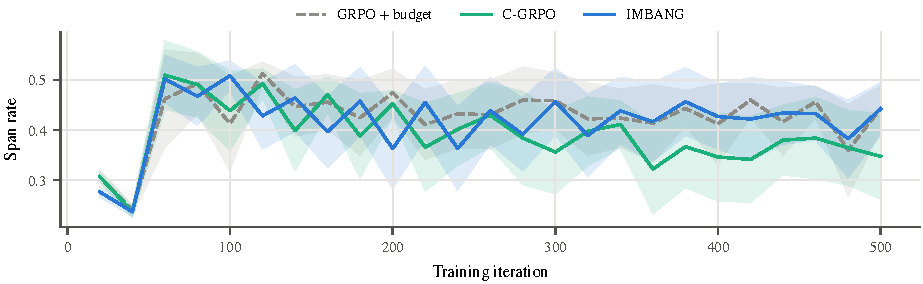
\includegraphics[width=0.85\textwidth]{figures/spanrate.pdf}
\caption{Span rate during training: share of groups whose members differ in outage count, averaged over all training contexts (mean and 95\% confidence band over ten seeds). The safe-side member does not raise this average; its effect is on the direction of the update (Section~\ref{sec:s-mech}).}
\label{fig:s-span}
\end{figure}

% ===========================================================================
\section{Per-Seed Results and Interpretability}
\label{sec:s-interp}
% ===========================================================================
Table~\ref{tab:s-seeds} lists, for each seed, IMBANG's Protocol~B results, its final validation outage rate and multiplier, the fidelity of the distilled depth-4 rule trees, and the certified PanicGuard constants. Seed~43 is the one run whose final validation outage rate (0.076) exceeds the budget. The focus tree of seed~42 is reproduced below as an example of the rules an operator can audit. Class 0 is source-address filtering and class 1 is protocol filtering; the threshold and drop trees are in the archive.

\begin{center}
\begin{minipage}{0.6\textwidth}
\footnotesize
\begin{verbatim}
|--- http_ratio <= 0.219
|   |--- class: 1
|--- http_ratio >  0.219
|   |--- packet_size_entropy <= 0.644
|   |   |--- class: 0
|   |--- packet_size_entropy >  0.644
|   |   |--- udp_ratio <= 0.086
|   |   |   |--- total_packet_rate <= 0.785
|   |   |   |   |--- class: 0
|   |   |   |--- total_packet_rate >  0.785
|   |   |   |   |--- class: 1
|   |   |--- udp_ratio >  0.086
|   |   |   |--- class: 1
\end{verbatim}
\end{minipage}
\end{center}

\begin{table}[!htbp]
\centering
\caption{IMBANG per Seed: Results, Budget, Rule Distillation and Certified Shield}
\label{tab:s-seeds}
\small
\resizebox{\textwidth}{!}{%
\begin{tabular}{@{}ccccccccccc@{}}
\toprule
Seed & Composite (B) & Severe (B) & Val.\ outage rate & Budget met & Final $\lambda$ & Focus acc.\ (\%) & Threshold MAE & Drop MAE & Leaves & PanicGuard gate / cap / floor \\
\midrule
42 & -0.241 & 11.0 & 0.021 & yes & 0.00 & 99.8 & 0.011 & 0.022 & 33 & 0.52 / 0.07 / 0.42 \\
43 & -0.233 & 20.1 & 0.076 & no & 0.10 & 100.0 & 0.014 & 0.016 & 29 & 0.54 / 0.08 / 0.42 \\
44 & -0.252 & 21.5 & 0.033 & yes & 0.00 & 99.8 & 0.010 & 0.023 & 34 & 0.50 / 0.14 / 0.29 \\
45 & -0.252 & 14.3 & 0.011 & yes & 3.63 & 99.2 & 0.007 & 0.021 & 36 & 0.50 / 0.10 / 0.41 \\
46 & -0.241 & 12.9 & 0.049 & yes & 0.00 & 99.5 & 0.022 & 0.017 & 32 & 0.47 / 0.05 / 0.39 \\
47 & -0.260 & 14.2 & 0.031 & yes & 0.04 & 99.8 & 0.006 & 0.007 & 31 & 0.54 / 0.20 / 0.36 \\
48 & -0.247 & 19.9 & 0.025 & yes & 0.00 & 99.8 & 0.026 & 0.021 & 30 & 0.60 / 0.10 / 0.40 \\
49 & -0.221 & 16.4 & 0.028 & yes & 0.46 & 99.8 & 0.010 & 0.015 & 32 & 0.51 / 0.07 / 0.41 \\
50 & -0.262 & 10.1 & 0.007 & yes & 0.02 & 99.9 & 0.012 & 0.019 & 36 & 0.53 / 0.18 / 0.37 \\
51 & -0.248 & 8.0 & 0.010 & yes & 0.00 & 99.9 & 0.008 & 0.010 & 30 & 0.54 / 0.10 / 0.40 \\
\bottomrule
\end{tabular}}
\vspace{2pt}
\parbox{\textwidth}{\footnotesize Rule distillation: depth-4 decision trees fitted to the final policy, evaluated on held-out states. PanicGuard defaults are 0.60 / 0.10 / 0.40.}
\end{table}


% ===========================================================================
\section{Simulated Operator for Zero-Shot ICMP Floods}
\label{sec:s-human}
% ===========================================================================
The letter notes that IMBANG has more severe outages than Sentinel under zero-shot ICMP floods, and that an operator applying Sentinel's ICMP constants closes the gap. Table~\ref{tab:s-human} gives the full study. It is a sensitivity analysis with a simulated operator, not a user study. The playbook constants are Sentinel's own ICMP override values, fixed a priori. With 90\% recognition accuracy the playbook lowers IMBANG's ICMP outages from 17.9 to 2.1 per 500 windows. The composite score falls slightly, from $-0.463$ to $-0.480$, because the fixed playbook filters less aggressively and leakage rises. The same operator also helps Sentinel (from 6.9 to 0.7), so the playbook narrows the difference between the two defenders rather than reversing it.

\begin{table}[!htbp]
\centering
\caption{Simulated Operator Applying Sentinel's ICMP Constants (Ten Seeds, 20 Episodes)}
\label{tab:s-human}
\small
\resizebox{\textwidth}{!}{%
\begin{tabular}{@{}llccccccc@{}}
\toprule
 & & \multicolumn{2}{c}{ICMP} & \multicolumn{2}{c}{ICMP-chaos} & \multicolumn{2}{c}{Strong} & \\
\cmidrule(lr){3-4}\cmidrule(lr){5-6}\cmidrule(lr){7-8}
Defender & Operator (accuracy) & Severe & Composite & Severe & Composite & Severe & Composite & Switches \\
\midrule
Sentinel & none & 6.9 & -0.480 & 28.2 & -0.332 & 159.6 & -0.753 & 0.0 \\
Sentinel & ICMP playbook, 0.7 & 1.7 & -0.481 & 28.2 & -0.334 & 161.8 & -0.756 & 4.2 \\
Sentinel & ICMP playbook, 0.9 & 0.7 & -0.481 & 28.2 & -0.334 & 160.6 & -0.754 & 2.2 \\
Sentinel & ICMP playbook, 1.0 & 0.3 & -0.482 & 28.1 & -0.334 & 159.6 & -0.753 & 1.0 \\
\midrule
IMBANG & none & 17.9 & -0.463 & 21.1 & -0.286 & 37.9 & -0.586 & 0.0 \\
IMBANG & ICMP playbook, 0.7 & 4.2 & -0.476 & 22.4 & -0.298 & 47.0 & -0.599 & 4.2 \\
IMBANG & ICMP playbook, 0.9 & 2.1 & -0.480 & 22.0 & -0.298 & 41.2 & -0.591 & 2.2 \\
IMBANG & ICMP playbook, 1.0 & 0.5 & -0.481 & 21.9 & -0.298 & 37.9 & -0.586 & 1.0 \\
\bottomrule
\end{tabular}}
\vspace{2pt}
\parbox{\textwidth}{\footnotesize Every ten windows a simulated operator recognises the active family with the stated accuracy and, after three windows, applies protocol filtering with drop 0.5 and threshold 0.5 during ICMP floods. This study draws its own traffic, so its no-operator rows differ slightly from Table~\ref{tab:s-b1}. Severe per 500 windows; switches: playbook changes per ICMP episode.}
\end{table}


% ===========================================================================
\section{Code, Data and Reproduction}
\label{sec:s-repro}
% ===========================================================================
The archive \texttt{IMBANG\_supplementary.zip} contains:
\begin{itemize}
\item the simulator port, the shield, the learners and the evaluation code;
\item the equivalence tests against Sentinel's reference implementation;
\item the per-seed result files behind every table and figure;
\item the trained checkpoints, ten seeds for each method in Table~\ref{tab:s-names} (champion and final networks, training logs, distilled rule trees and certified shield constants);
\item this document.
\end{itemize}
Sentinel's checkpoints are not redistributed; they are available from its public repository~\cite{sentinelcode}. The archive's \texttt{README.md} maps every table and figure to the script and data file that produce it. In brief:
\begin{itemize}
\item \texttt{pytest tests} checks the port;
\item \texttt{scripts/nl\_assets.py} and \texttt{scripts/supp\_assets.py} regenerate the tables and figures from the included results in under a minute;
\item \texttt{scripts/evaluate.py} re-evaluates the included checkpoints under Protocols A--C;
\item \texttt{scripts/train.py} retrains a method.
\end{itemize}
One training run takes 3--5 minutes on a single CPU core. The full grid of ten methods and ten seeds takes about 6--8 CPU-hours. Evaluation is deterministic: re-running Protocol~B on the included checkpoints reproduces Tables~\ref{tab:s-b1}--\ref{tab:s-b2} exactly.

\textbf{Scope.} All results come from Sentinel's simulator, not from production traffic. The simulator and shield port are derived from Sentinel's MIT-licensed code~\cite{sentinelcode}.

\bibliographystyle{IEEEtran}
\bibliography{../refs}

\end{document}
